\section{Jackson und das Jackson Projekt}
Das Jackson Projekt entwickelt eine freie und modulare Bibliothek f\"ur die Serialisierung und Deserialisierung von Java-Instanzen in \ac{JSON}-Dokumente. Jackson wird unter der Contributor License Agreement (CLA) vermarktet. Die zur Zeit aktuelle Version ist 2.4.1, welche auch bei der Bearbeitung des Projektes eingesetzt wird.

\subsection{Jackson-Module}
Die Jackson-Bibliothek besteht aus drei Hauptmodulen, welche wie folgt bezeichnet sind:
\begin{itemize}
 \item "`jackson-core"' welches die JSON spezifische Implementierung sowie eine low-level streaming API enth\"alt
 \item "`jackson-annotations"' welches die Jackson spezifischen Annotationen enth\"alt.
 \item "`jackson-databind"' welches f\"ur das \textit{databind} verantwortlich ist.
\end{itemize}
Unter Databind wird eine Methode verstanden, welche \"uber ein User-Interface gesteuert werden kann.
Diese Methode ist in der Lage Daten aus einem Datenstrom wie zum Beispiel einem JSON-File zu lesen oder zu schreiben.

Mit diesen drei Modulen ist Jackson voll einsetzbar und kann Java-Instanzen zu einem JSON-Datenstrom umwandeln. Der JSON-Datenstrom wiederum kann gespeichert oder an andere Programme gesendet werden.

Um jedoch einheitliche Annotationen f\"ur Jackson und JAXB zu haben, wird ein weiteres Jackson-Modul ben\"otigt, welches in der Lage ist die JAXB-Annotationen zu verarbeiten.\cite{Jackson}

\subsection{Serialisierung mit Jackson}\label{Serialisierung}
Um eine Serialisierung mit Jackson umzusetzen wird zuerst eine Instanz der Klasse \texttt{ObjectMapper} ben\"otigt, welche den Databinder darstellt. Der \texttt{mapper} ist somit f\"ur die Convertierung von Java-Instanzen zu JSON-Dokumenten verantwortlich. 

Jedoch wird nicht nur der "`Converter"' ben\"otigt, sondern auch ein \texttt{AnnotationInspector}. Der \texttt{inspector} wird als Instanz von \texttt{JaxbAnnotationInspector} erstellt, welchem eine \texttt{TypeFactory} mit "`Default-Einstellungen"' \"ubergeben wird. Dies bedeutet es wird auf die Original JAXB-Annotationen geparst, ohne auf Sonderf\"alle zu achten. Andere Annotation werden nicht ber\"ucksichtigt. Der \texttt{inspector} wird nun dem "`Converter"' \"ubergeben, damit dieser auf die entsprechnden Annotationen reagieren kann.

Um eine \textit{Minimale Exception Safety} zu garantieren wird nun eine \texttt{Null}-Abfrage des zu serialisierenden Elements gemacht. Mit dieser Stufe der Sicherheit soll nicht verhindert werden das eine Exception passiert. Es wird lediglich garantiert das die Methode ohne Abzust\"urzen durchlaufen werden kann. \cite{ExceptionSafety}

Ist die zu serialisierende Instanz \texttt{Null} so wird eine \texttt{IllegalagumentException} generiert und die Methode so ordnungsgem\"a\ss{} beendet. Ist eine Instanz vorhanden, wird diese dem \texttt{mapper} \"ubergeben. Das Ergebnis des Aufrufs von \texttt{writeValueAsString} ist entweder bei Erfolg ein valider JSON-String oder beim scheitern eine \texttt{JsonProcessingException}.

Dieser Zusammenhang ist noch einmal im folgenden Quellcode-Beispiel beschrieben.
\newpage
\lstinputlisting{Code/Jackson_bsp.java}

\subsection{Deserialisierung mit Jackson}
F\"ur die Deserialisierung mit Hilfe von Jackson wird wie bei der Serialisierung ebenfalls ein Databinder und AnnotationInspector ben\"otigt, welche wie im Kapitel \ref{Serialisierung} erstellt werden. 

Bevor dies jedoch passiert, wird gepr\"uft ob der eingegebene String weder \texttt{Null} noch \texttt{Empty} ist. 
Sollte das der Fall sein, wird die Methode \texttt{readValue} mit dem \"ubergebenden String und der Information um welche Klassen-Instanz es sich beim String handelt \"ubergeben.

Die Schwierigkeit beim Deserialisieren besteht also nun darin, das bevor der String \"uberhaupt deserialisiert werden kann erst festgestellt werden muss um welche Klasse es sich eigentlich handelt.

Im Codebeispiel unten wird momentan noch davon ausgegangen, das es sich immer um eine Instanz der Klasse "`TestData"' handelt. Wie diese Einsch\"ankung aufgehoben werden kann wird im folgenden Kapitel beschrieben.

\lstinputlisting{Code/Jackson_des_bsp.java}
\subsection{Klassendiagramm der Serialisierung}

Wie von OPM verlangt erben hier alle Klassen von OPMObject. Um diese Arbeit mit der von Herrn Achim Walz vergleichen zu k\"onnen wurde sich auf eine gemeinsame abstrakte Klasse \texttt{Serializer} geeinigt. 

Die Klasse \texttt{JSONSerializer} erbt um einen Direkten vergleichen durchf\"uhren zu k\"onnen genau wie \texttt{XMLSerializer} von \texttt{Serializer}.
\texttt{Testdata} und \texttt{TestData2OPM} sind erste Test-Klassen von denen Instanzen serialisiert und deserialisiert werden.

Main-Klasse in diesem Projekt ist \texttt{OPM\_Serializer}. Die \texttt{main}-Methode setzt die Serialisierung im Test in Gang.

Damit wie gew\"unscht jede Klasse serialisiert werden kann, wurde die Methode \texttt{serializeMe} zu OPMObject hinzugef\"ugt.
Diese Methode nutzt nun bei Aufruf die \texttt{serialize}-Methode des jeweiligen Serialisierers.

Ein vollst\"andiger \"Uberblick ist im Klassendiagramm unten zu finden gegeben.

\FloatBarrier
\begin{figure}[ht]
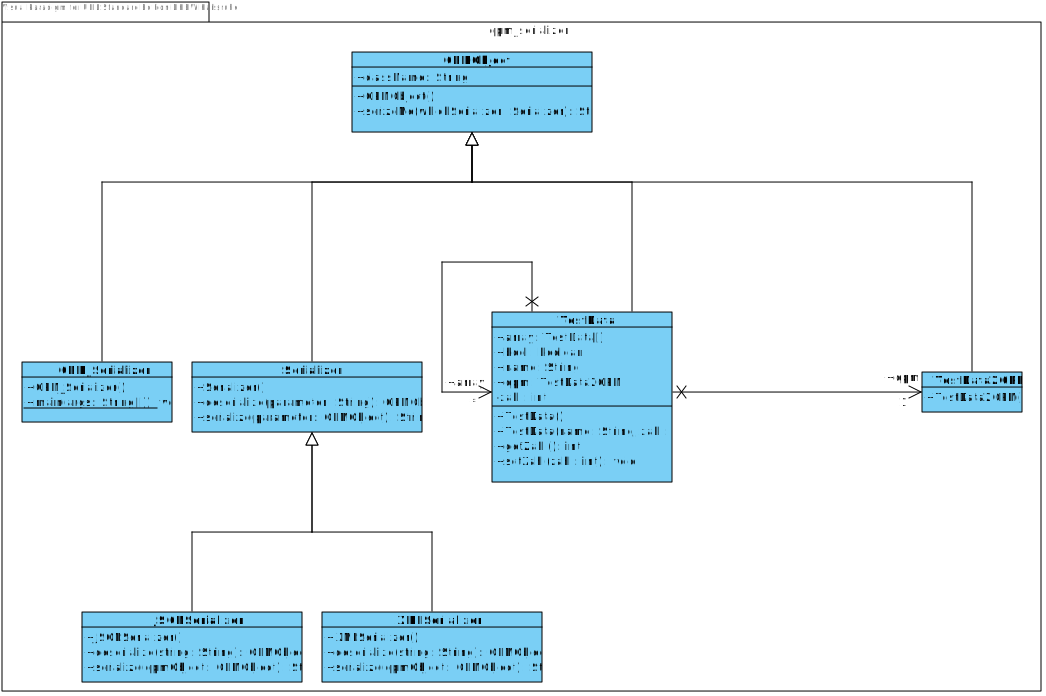
\includegraphics[width=16cm]{Bilder/Erstes_EKD}
\label{Klassendiagramm der Serialisierung}
\caption{Klassendiagramm der Serialisierung} 
\end{figure}

\subsection{JSON-Schema Erstellung aus einer Klasse}\label{JSON-Schema}
\"Ahnlich bei auch bei XML gibt es in JSON ein Datenformat, welches die zu erwartende Form des Streams vorgibt.
Wie auch in XSD wird das Schema in der eigenen Norm als konformes Dokument erstellt. \cite{JSON_Schema}

Ein Beispiel f\"ur ein JSON-Schema wird hier Anhand des JSON-Dokuments in Kapitel \ref{Der Aufbau von JSON} dargestellt.
Das JSON-Schema besteht aus einem Objekt, welches die jeweiligen Namen und Werte der Attribute einer Instanz enth\"alt.

Somit steht am Anfang eines JSON-Schemas immer der Bezeichner \texttt{type} mit dem entsprechenden Wert, n\"amlich \texttt{object}.
Unter dem Schl\"ussel \texttt{properties} sind wiederum als inneres Objekt die Attribute mit ihren m\"oglichen auspr\"agungen aufgelistet. 

Am Anfang einer Propertie steht der Attributname \texttt{"}\texttt{String"}, wie im Beispiel unten.
Gefolgt wird dieser Name von einem Objekt, welches die genauen Eigenschaften des Attributs beschreibt.
Im Beispiel wird einfach nur der Typ des Attributs bezeichnet, jedoch ist auch m\"oglich weitere Einschr\"ankungen \"uber Annotationen zu machen. Mit dessen Hilfe k\"onnte man zum Beispiel einen Wertebereich f\"ur Zahlen angeben.

Um die XML-Annotationen von JAXB bei der Schemaerzeugung zu nutzen muss wieder ein \texttt{AnnotationInspector} verwendet werden.

Die Einschr\"ankungen und Beschreibungen der Attribute werden dem Serializer mit Hilfe der Annotationen \"ubergeben, welche Java-Methoden-Namen enthalen . Das setzen der Beschreibungen geschieht \"uber Java-Methoden welche zur Laufzeit vom Serializer aufgerufen werden.

Auf die Erkl\"arung der einzelnen Annotationen von JAXB wird an dieser stelle verzichtet, da dieses Thema zu Umfangreich ist um es in dieser Arbeit abzuhandeln. 

\lstinputlisting{Code/JSON_Schema.json}

\subsection{JSON-Schema mit Hilfe von Jackson erstellen}
Seit der Jackson Version 2.2 wurde das Modul zur Erstellung eines JSON-Schemas aus dem Modul "`jackson-databind"' ausgegliedert und ein eigenes Modul mit erweitertem Funktionsumfang eingef\"uhrt. 

F\"ur die Erstellung eines JSON-Schemas wird somit das Zusatzmodul \\"`jackson-module-jsonSchema"' ben\"otigt. Um unn\"otige Fehlerquellen zu vermeiden wurde auch dieses Modul in der Version 2.4.1 verwendet, auch wenn es zum Erstellungsdatum schon eine neuere Version gab. Somit sind alle Module von der selben Version und Fehler durch Versionsunterschiede sind ausgeschlossen.

Wie schon in fr\"uheren Beispielen gezeigt wird zu erst wieder ein \texttt{ObjectMapper} erstellt. Hierbei kann eine JsonMappingException auftreten, welche entweder weiter gewurfen werden kann oder dirket behandelt wird.
Des weiteren wird f\"ur die Schemaerzeugung noch ein \\\texttt{SchemaFactoryWrapper} erstellt, welcher das Schema erstellt.
Der Schema-Wrapper kann unter umst\"anden die JsonProcessingException werfen.

Dem Wrapper wird nun \"uber den n\"achsten Methodenaufruf auf den Mapper und die entsprechend zu Mappende Instanz angesetzt. Dies geschieht \"uber die Methode \\\texttt{acceptJsonFormatVisitor}.

Mittels der Methode \texttt{finalSchema} wird das Schema der Instanz als \texttt{JsonSchema} erstellt.

\"Uber den \texttt{return}-Wert wird das \texttt{JsonSchema} als String \"ubergeben.

Im Codebeispiel unten wird dieser Zusammenhang noch einmal verdeutlicht.

\lstinputlisting{Code/generateSchema.java}

\subsection{Auff\"alligkeiten beim Testen}
Beim Serialisieren und Deserialisieren sollen Attribute in JSON-Dokumenten gespeichert werden. Hief\"ur ben\"otigen alle Klassen einen Standard-Konstruktor damit der Serializer diesen Aufrufen kann. 

Des weiteren ben\"otigt der Serializer f\"ur alle nicht \texttt{public} Attribute Getter- und Settermethoden um Zugriff auf diese Attribute zu erhalten. Denn der Serializer darf durch Java-Richtlinien nur auf \texttt{public} Attribute ohne Getter- und Settermethoden zugreifen.

Um eine Serialisierung von allen Klassen zu gew\"arleisten muss eventuell das OPM-Modell angepasst werden.
Da alle Klassen sich an die OPM-Regeln halten, ist somit gew\"ahrleistet das alle ankommenden Instanzen serialisiert oder deserialisiert werden k\"onnen.

In ersten Tests mit dem JSONSerializer wurde die Funktionsf\"ahigkeit bewiesen. Jedoch ist der derzeitige Stand des Serialisierers noch nicht in der Lage verschiedene Klassen zu deserialisieren. Bisher ist der Klassenname fest vorgebeben.

Im Projekt aber sollen unterschiedlichste Klassen deserialisiert werden k\"onnen. Das wirft die Frage auf wie Festgestellt wird, um welche Klasse es sich bei der Instanz handelt. Dieser Punkt wird nun in den folgenden Kapiteln ausf\"uhlich erl\"autert.

\subsubsection{Auff\"alligkeiten beim erstellen des JSON-Schemas}
Nach einigen Tests wurde festgestellt, das Jackson f\"ur alle Zahlen immer \texttt{integer} im Schema angibt, obwohl JSON auch \texttt{double} oder \texttt{float} kennt. Egal ob es sich in der Klasse um \texttt{float, double} oder  \texttt{integer} handelt. Warum dies im Schema nicht Ordnungsgem\"a\ss{} \"ubernommen wird, konnte nach einiger recherche nicht herausgefunden werden.